% -*- mode: latex; mode: auto-fill; coding: utf-8; -*-

The main advantage of representing an implicit counture or surface as
a signed distance field, is that the length of the gradient is
one. This is also exactly what defines a signed distance field.

When constructing or manipulating a signed distance field defined on a
Cartesean grid, the result is not always signed distance field. So to
enable further calculations or iterations of an algorithm the result
must be turned into a new signed distance field that reflexts the
changes done by the calculations. This process is called
\dit{reinitialization} of the level set, and can be done several
different ways.

Algorithms to reinitializing signed distance fields focuses on
reinitializing the whole domain, and at the same time keeping the zero
level set as fixed as possible. This means that the process disrupts
data outside the zero level set, which depending on the type of
phemomena we are modelling can be problematic. For the problems we are
modelling this is not an issue, and is therefore not of relevance here.

Before diving into the algoritms a good question is, how often must the
level set be reinitialized? There is no good answer to this question,
because it depends on how rapidly the contour is changing. In our work
we have been reinitializing after ever change, which ensures that this
is not a source of error.

The two most used algoritmic approched to reinitialization are:
geometricly methods that calculations distances to the contour or surface,
and PDE based methods that numerical approximates solutions to the Eikonal
equation: $||\nabla \phi|| = 1$ \citbook{bridson2008fluid}{page~89}.

When initializing the implicit contour in section \vref{sec:initialization}
we used an algorithm that geometricly calculated the distance to the
contour. So the natural choise should be also to use this algorithm for
reinitializing, but because the algorithm does not calculate the
signed distance function precise enough, we cannot use this algorithm
when reinitializing. Furthermore if we had used this type of
algorithm, the we would have had to construct the contour before
invoking the algorithm. Constructing the contour is very expensive,
and is something that should be avoided at almost all cost when using
the level set method.

Instead we have chosen to use PDEs to solve the Eikonal
equation. Solving the Eikonal equation can also be done in different
ways, which we will describe in the next subsections.

\subsection{The PDE way of reinintalizing}
When using the PDE way of reinitialing the level set, we solve the
following PDE \citbook{osher2002level}{page~65-66}:

\begin{equation}
\label{eq:reinit}
\phi_t + S(\phi_0)(|\nabla \phi| - 1) = 0
\end{equation}

Where $\phi$ is the SDF being evolved as a PDE, and $\phi_0$, is the
initial SDF giving as input to the reinitialization algorithm, which
has not been altered by the process of solving the PDE. The function
$S(\phi_0)$ gives the sign of the SDF, like the following function,
described in \citbook{osher2002level}{page~66}:
%\citbook{article:FLLSM}{page~419}:

\begin{equation}
\label{eq:s1}
S(\phi) =
\begin{cases}
-1 &\mbox{ if } \phi < 0, \\
 0 &\mbox{ if } \phi = 0, \\
 1 &\mbox{ if } \phi > 0.
\end{cases}
\end{equation}

When using this approach of reinitializing the SDF, then the grid
points in $\phi$ that are nearest to the contour is reinitialized
first, and then propergated in the normal direction from the zero
level set, hereby reinitializing the grids points in layers each
iteration.

This algorithm is relatively slow if all grid points needs to be
reinitialized, because it only reinitializes one layer in each
iteration when solving the PDE. This means that the PDE, on a
two-dimensional domain, must be iterated
$\sqrt{width^2 \times height^2}$ times to make sure that the algoritm
has reinitialized the whole domain.

But because the algorithm has the property of reinitializing the SDF
in layers it is of special interest in reguards to performance when
using a narrow band level set as described in section
\vref{sec:narrowband}. Here only three or four layers around the SDF needs
to be reinitialized, making the algorithm ideal for the narrow band
approach.

\subsection{The sign function S}
Because equation \ref{eq:reinit} is a hyperbolic PDE, we need to use a
smeared out version of equation \eqref{eq:s1}. One way of smearing the
function is to using equation \eqref{eq:Sphi0}.

\begin{equation}
\label{eq:Sphi0}
S(\phi_0) = \frac{\phi_0}{\sqrt{\phi_0^2 + (\Delta x)^2}}
\end{equation}

The difference between equation \eqref{eq:s1} and equation
\eqref{eq:Sphi0}, can more easily be seen be looking at a plot of the
two functions, as depicted in figure \ref{fig:s-graph}.

\begin{figure}[h]
\begin{center}
  \subfloat[Plot of equation \eqref{eq:s1}]{
    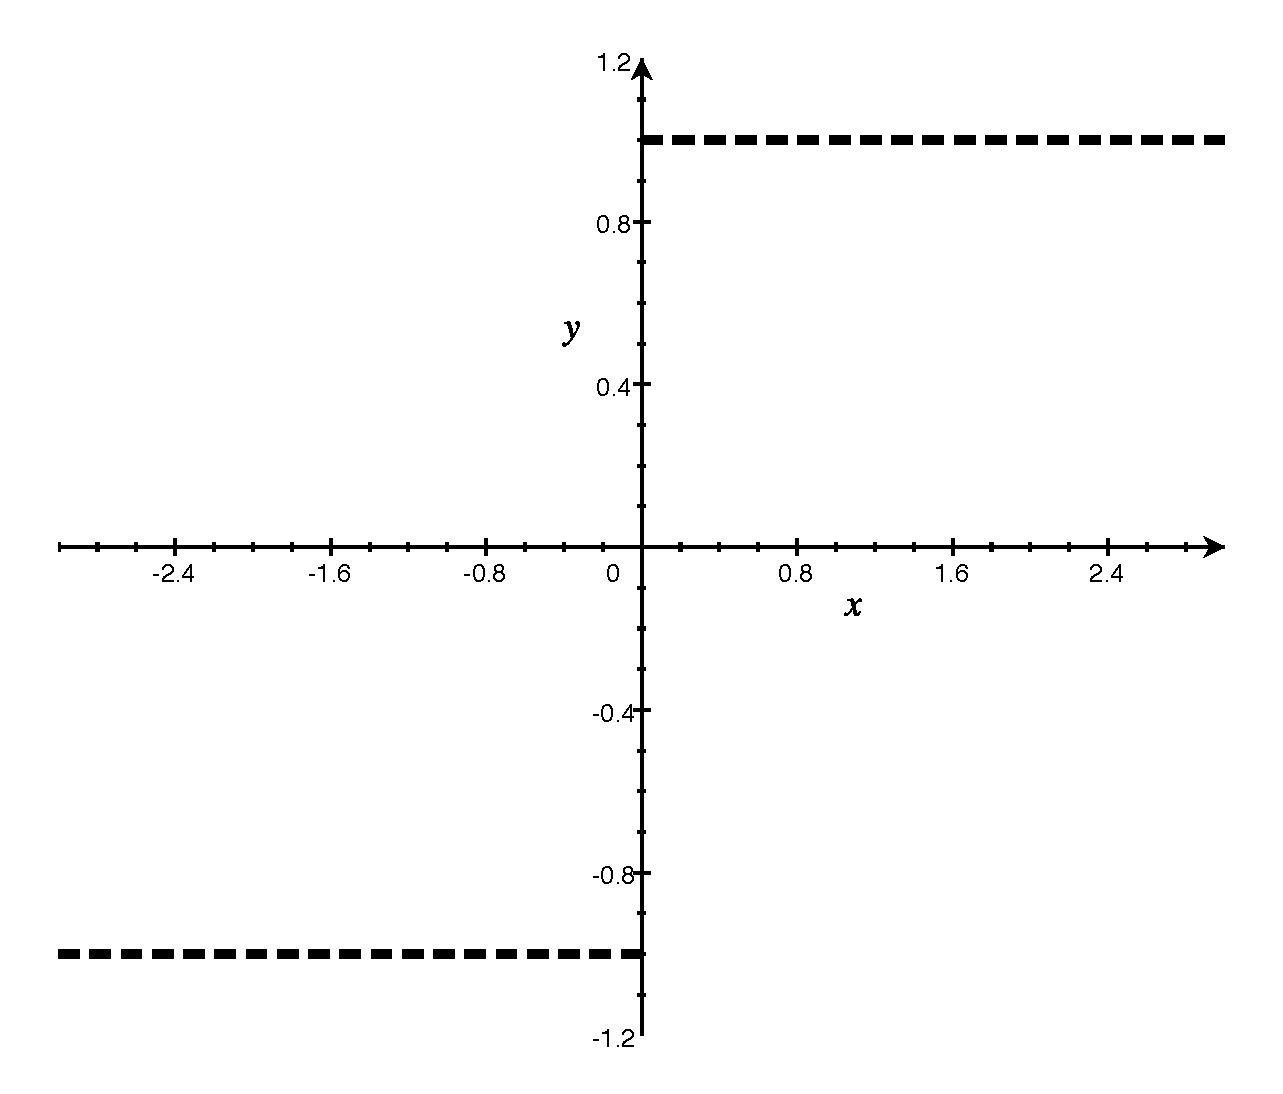
\includegraphics[width=0.5\textwidth]{imgs/S0.pdf}
    \label{fig:fake1}
  }
  \subfloat[Plot of equation \eqref{eq:Sphi0}, $\Delta x=1$]{
    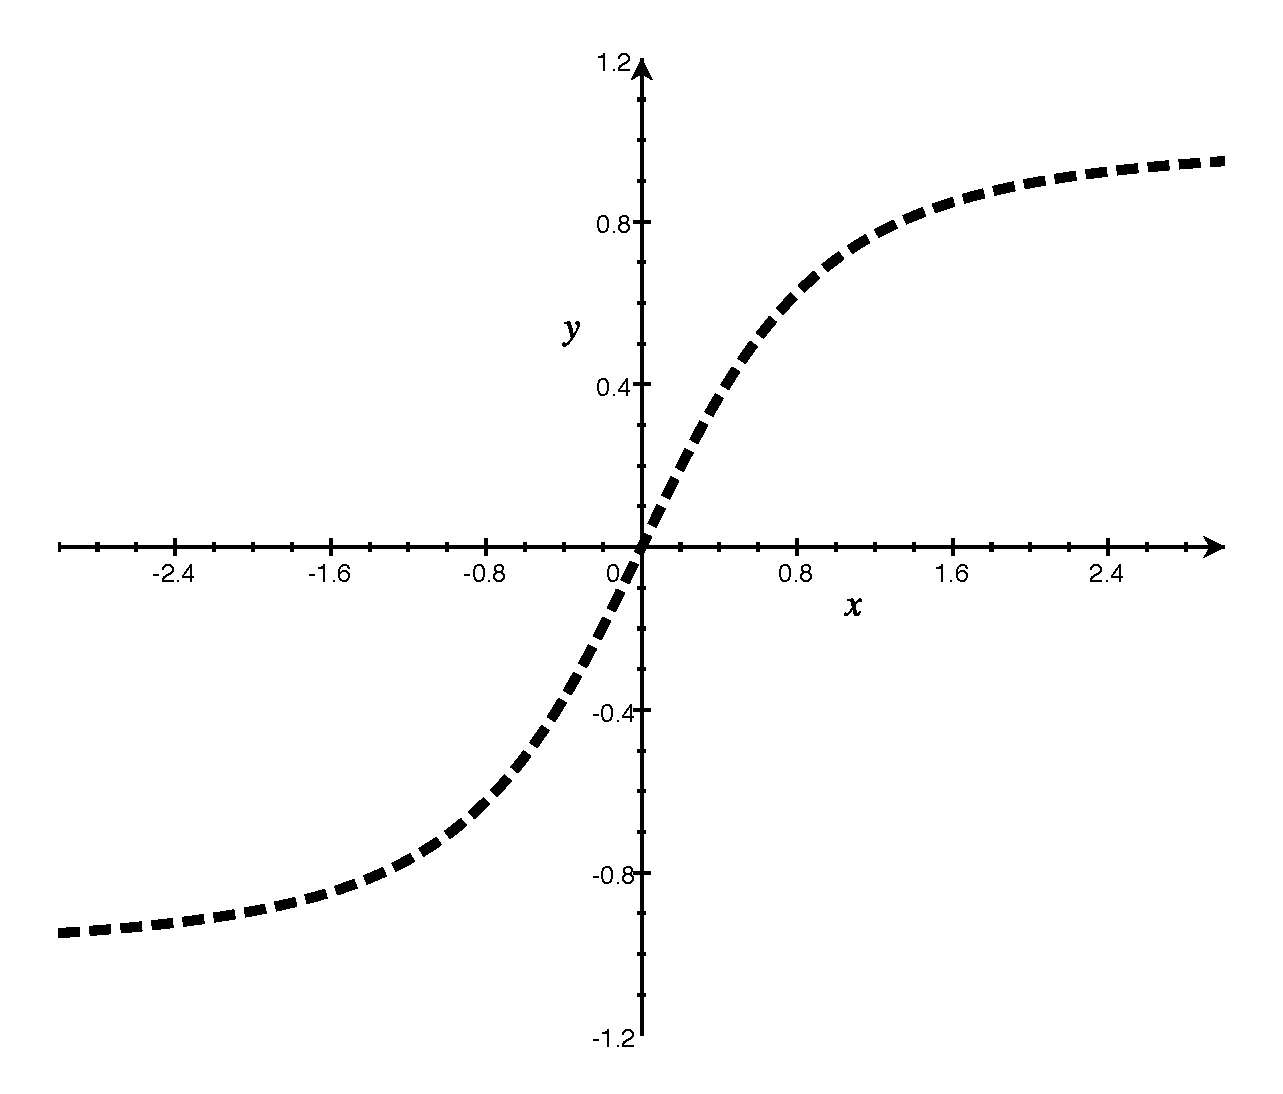
\includegraphics[width=0.5\textwidth]{imgs/S1.pdf}
    \label{fig:fake2}
  }
\end{center}
\caption{Illustrations of S}
\label{fig:s-graph}
\end{figure}

%\subsection{CFL-condition}


\pagebreak
\subsection{Implementation}
The implementation of how to solve the PDE in equation \eqref{eq:reinit},
uses the describtion of Godunov's scheme from
\citbook{osher2002level}{page~58} in the spatial dimensions, and a
forward Euler in the temporal dimension, as described in formular
(1.3) in \citbook{osher2002level}{page~10}.

\begin{lstlisting}[language=c++]
    Tex<float> phi0 = GetPhi(); Tex<float> phin = GetPhi();
    for (unsigned int i = 0; i<iterations; i++) {
        for (unsigned int x = 0; x < width; x++) {
            for (unsigned int y = 0; y < height; y++) {
                float xy = phi(x, y);                
                float phiXPlus = 0.0f;
                float phiXMinus = 0.0f;
                float phiYPlus = 0.0f;
                float phiYMinus = 0.0f;        	
                if (x != width-1) phiXPlus  = (phi(x+1, y) - xy);
                if (x != 0)       phiXMinus = (xy - phi(x-1, y));
                if (y !=height-1) phiYPlus  = (phi(x, y+1) - xy);
                if (y != 0)       phiYMinus = (xy - phi(x, y-1));
        	
                float dXSquared = 0;
                float dYSquared = 0;
                float a = phi0(x,y);
                if (a > 0) {
                    // formula 6.3 page 58
                    float max = std::max(phiXMinus, 0.0f);
                    float min = std::min(phiXPlus, 0.0f);
                    dXSquared = std::max(max*max, min*min);
                    max = std::max(phiYMinus, 0.0f);
                    min = std::min(phiYPlus, 0.0f);
                    dYSquared = std::max(max*max, min*min);
                } else {
                    // formula 6.4 page 58
                    float max = std::max(phiXPlus, 0.0f);
                    float min = std::min(phiXMinus, 0.0f);
                    dXSquared = std::max(max*max, min*min);
                    max = std::max(phiYPlus, 0.0f);
                    min = std::min(phiYMinus, 0.0f);
                    dYSquared = std::max(max*max, min*min);        				
                }
                float normSquared = dXSquared + dYSquared;           
                float norm = sqrt(normSquared);

                // Using the S(phi) sign formula 7.6 on page 67
                float sign = phi0(x,y) / sqrt(phi0(x,y)*phi0(x,y) + 1);
                float dt = 0.3; // A stabil CFL condition
                phin(x,y) = phi(x,y) - sign*(norm - 1)*dt;
            }
        }
        for (unsigned int y=0; y<height ; y++)
            for (unsigned int x=0; x<width; x++)
                phi(x,y) = phin(x,y);

    }
\end{lstlisting}
